% Shared preamble for the English summaries in this repository.
\documentclass[11pt,a4paper]{article}
\usepackage[margin=2.2cm]{geometry}
\usepackage[T1]{fontenc}
\usepackage[utf8]{inputenc}
\usepackage{lmodern}
\usepackage{amsmath,amssymb}
\usepackage{graphicx}
\usepackage{booktabs}
\usepackage{enumitem}
\usepackage[hidelinks]{hyperref}
\setlist{itemsep=2pt,topsep=4pt}
\setlength{\parindent}{0pt}
\setlength{\parskip}{5pt}
\graphicspath{{figures/}}
\newcommand{\summaryheader}[3]{%
  \begin{center}
    {\Large\bfseries #2}\\[3pt]
    {\large #1}\\[3pt]
    {\small Arshia Goshtasbi \textbullet{} MSc Electrical Engineering (Control), Iran University of Science and Technology \textbullet{} #3}
  \end{center}
  \vspace{2pt}\hrule\vspace{8pt}
  \noindent\textit{English summary of my original Persian report, which is kept as a PDF in this folder.}\par}

\begin{document}
\summaryheader{Adaptive Control, Homework 4}{Self-tuning Regulators under Disturbances (Åström \& Wittenmark, Examples 3.9 and 3.10)}{Autumn 1404 (2025)}

All cases are subsystems of \texttt{HW4.slx}. I compared three versions of the self-tuning regulator when a load disturbance acts on the plant.

\begin{description}
  \item[1. Standard STR (example 3.9).] Very sensitive to the disturbance. The noise enters the RLS estimator, so the estimates oscillate, the output has ripple, and the control signal is jumpy.
  \item[2. STR with filtered signals $u_f$, $y_f$ (example 3.10).] Filtering the regression signals gives the estimator cleaner data. The estimates oscillate less, the control is smoother and tracking improves, but the disturbance is not fully removed.
  \item[3. STR with a disturbance model (example 3.10, modified).] The disturbance dynamics are included in the model, so the estimator learns them along with the plant. This gives the best tracking, the steadiest estimates and a smooth control signal, and is almost unaffected by the disturbance.
\end{description}

\begin{center}
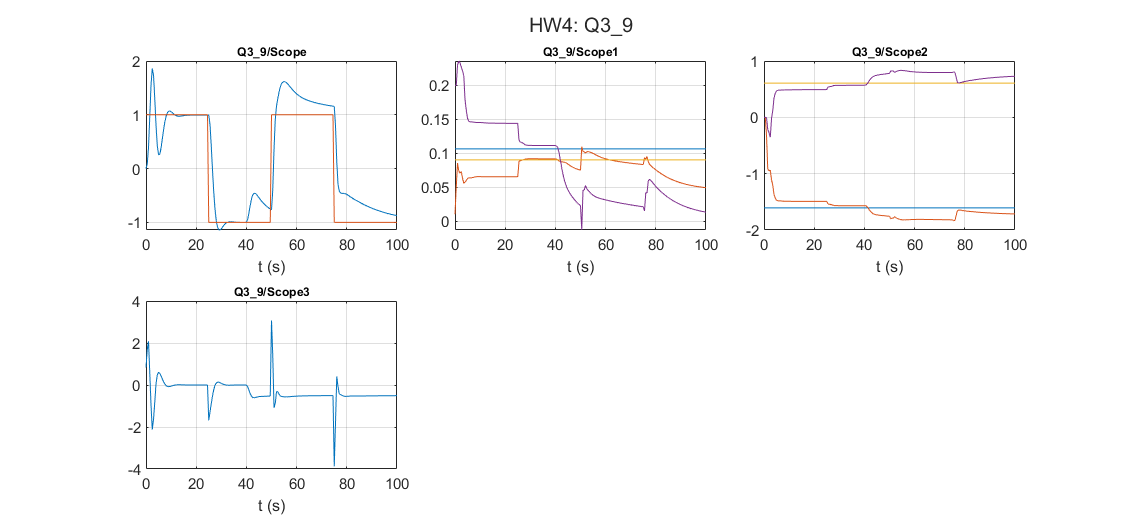
\includegraphics[width=0.9\linewidth]{Q3_9.png}\\[2pt]
{\small Re-run in R2023b: example 3.9, the standard STR under a disturbance.}
\end{center}
\end{document}
